\chapter{序論}
\section{はじめに}
1953年、James WatsonとFrancis Crickは、遺伝情報の実体は4種類のデオキリボ核酸が相補的に水素結合した二重らせん構造であること鮮やかに示した \citep{watson1953molecular}。5年後の1958年、F. Clickは"Ideas for protein synthesis"  (図\ref{fig:crick_idea})において、遺伝情報はDNA-RNA-タンパクへと一方向性を持って伝達されるという着想を得ており、1970年には分子生物学におけるセントラルドグマ (中心原理)を提唱した \citep{crick1970central}。1960年代から70年代には、Marshall NirenbergやSydney Brennerなど多くの研究者により、コドンの発見と遺伝暗号が解読されると、塩基配列がアミノ酸を表現する基本原則が明らかとなった。黎明期における分子生物学は、物理学者が多く参入した経緯も相まって、分子のことばで生命の持つ普遍的性質の理解を標榜する学問として誕生し、熾烈な競争の下に急速な進展を遂げた。

\begin{figure}[!h]
	\begin{center}
		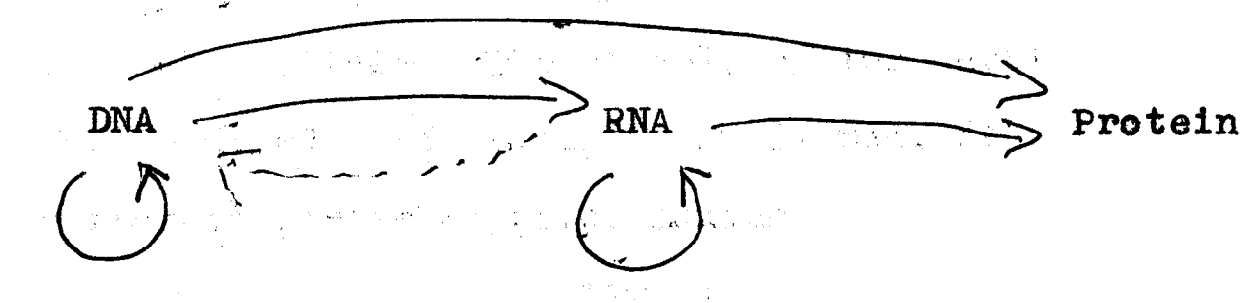
\includegraphics[width=15cm]{crick_idea.png}
	\end{center}
	\caption{\small{\textit{"Ideas on Protein Synthesis"}に描かれたセントラルドグマのアイデア。矢印の方向は、遺伝情報の流れを表している。破線はRNAからDNAへ向いており逆転写酵素を予見させるが、クリックが1958年当時に想定していたかは定かでない。}}
	\label{fig:crick_idea}
\end{figure}

分子生物学は生命の普遍性を明らかにする過程で、内在的に多様性を生み出す数々の機序をも明らかにしてきた。1970年、Howard TeminおよびDavid Baltimoreは一本鎖RNAを鋳型として、相補的なDNAを合成する逆転写酵素を発見した \citep{TemMiz7006,Bal7006}。この発見は、セントラルドグマから逸脱し、RNAからDNAへも遺伝情報は伝達しうることを示した画期的な発見であった。その後も、真核生物における遺伝子はスプライシング機構によってイントロンが切り出され複数のエクソンから構成されること \citep{ChoGelBro7709}、転写直後の新生RNAは3'末端にポリアデニル化 \citep{EDMABR6004}、5'末端にはキャップ構造が付加されて成熟すること \citep{WeiGerMos7504}、線虫からはコドンが異なるアミノ酸をコードする例外が発見されるなど \citep{HamFujMas1204}、セントラルドグマの概念もまた時代とともに拡張されてきた。このことは、本質的には、生命が逸脱や例外を含む多様性を担保する存在であることに他ならない。生命の持つ普遍的な性質の理解を目指した分子生物学において、多様性という個別的な生命現象をその対象することが逆説的には、生命の理解へと接続される重要なアプローチの一つだと私は考えている。
%\par
%転写はゲノム上にコードされた遺伝情報をRNAへ正確にコピーする機構を指す。転写は核内で起こる生化学反応であり、RNAポリメラーゼよって触媒される。転写されたpre-mRNAはスプライシング、ポリアデニル化と5'キャップ付加を受けて成熟した後に、核膜孔を通して細胞質へ輸送される、というのが転写機構の大まかな素描である。ヒトゲノムの解読前、遺伝子数はおよそ10万個だと見積もられていたが、2004年の完了宣言では2.5万個程度に大きく下方修正され、直感的な生命の複雑性と遺伝子数には直接の相関関係が見られないことは今日に繰り返すまでもない。
\par
真核生物の多様で複雑なシステムは、セントラルドグマからの逸脱の他に塩基やタンパク質への修飾が生命活動に不可欠であることは、現在の分子生物学においては前提となっている。細胞の内外の情報伝達には、キナーゼによるタンパク質のカスケード的なリン酸化反応が用いられ、リン酸化された分子が核内に移行し転写因子の活性を調節することで遺伝子発現の状態と量が制御される \citep{Boulikas:1995rm}。ヒストンは、アセチル基やメチル基による化学修飾を受け、染色体構造の変化を伴った遺伝子発現の調節や細胞の分化状態が決定されるなど \citep{Shilatifard:2006rt}、修飾の持つ生体内機序の制御例は枚挙にいとまがない。真核生物は、有限個の遺伝子にその種数を規定されながらも、転写および翻訳機構への修飾が多様性の生成を駆動する原動力であると言えるだろう。
\par
RNA編集 (RNA editing)は、転写後修飾 (Post-transcriptional modification)の一種である。RNA 
編集は、DNAにコードされた遺伝情報がRNAポリメラーゼにより転写された直後、RNAが別の塩基に修飾される現象を指す \citep{Wulff:2010aa}。RNA編集を受けた転写物は、元来の遺伝情報とは異なった配列情報を持つこととなり、こういった意図的な修飾は、DNAから正確なコピーとしてのRNAを合成するという転写機構からの逸脱と解釈することができる。興味深いことにヒトやマウス、ショウジョウバエといった高等真核生物においては、特定の遺伝子領域内へRNA編集を起こし、タンパク活性の変化や機能の調節に積極的に利用されているとの報告が蓄積している \citep{Pullirsch:2010aa}。また、ここ数年の超並列シーケンサー (High-throughput sequencing)によるトランスクリプトームの網羅的かつ定量的な計測は、非翻訳RNAや遺伝子間領域などこれまで研究対象とされなかった転写領域におけるRNA編集に光をあてており、非翻訳領域におけるRNA編集の生物学的な意義にも、今日大きな注目が集まっている \citep{Nishikura:2006aa, Nis10}。しかしながら、超並列シーケンサーを用いた情報学的なRNA編集サイトの検出や解析は、ここ数年に立ち上がった新しい領域であることから、一度の実験で得られる膨大なシーケンスデータから精度よく編集サイトを同定する手法とその機能解析に、確立された手法は未だ登場していない。
\par
本論文は、大きく4つの内容を取り扱う。第一章では、既往の研究により明らかにされてきたRNA編集機構の多様な生理学的な機構を概観するほか、超並列シーケンサーを用いた編集サイトの検出手法の発展について概説する。
第二章では、既存のRNA編集検出手法について性能評価を行い、高精度な検出に寄与する検出手法とそのパラメータについて議論する。第三章では、精度よく高速にRNA編集サイトを検出するソフトウェア・パッケージの開発を行った。第四章では、ヨコヅナクマムシのシーケンスデータから編集サイトを検出し、その情報学的解析を行った。本研究は、超並列シーケンサーから得られる大量のシーケンスデータを用いたRNA編集サイトの簡便な検出を可能にし、真核生物における転写後修飾とその制御機能の更なる解明に貢献することを期待するものである。

\newpage

\section{真核生物におけるRNA編集とADARの役割}
\subsection{転写後修飾機構としてのRNA編集}
RNA編集は転写物への一塩基修飾を指し、鞭毛虫のミトコンドリアから初めて発見された \citep{BenVanBra8609}。真核生物では、ADAR (Adenosine deaminase acting on RNA)によるアデニン(A)からイノシン(I)へ修飾されるA-to-I編集、APOBEC (Apolipoprotein B mRNA editing enzyme, catalytic polypeptide-like)によるシトシン (C)からウラシル (U)へのC-to-U編集がこれまで報告されている \citep{BenVanBra8609}。APOBECのターゲットとなる遺伝子は非常に少なく、ヒトではAPOBとNF1遺伝子のみが知られている \citep{CapFreSku9702}。
植物においては主にシロイヌナズナのミトコンドリアや色素体において、PPR (pentatricopeptide repeat)タンパクファミリーによるC-to-U編集が知られる \citep{Shi0603, MenCheJin10}。ヒトやマウス、ショウジョウバエにおいては、高頻度にA-to-Iへの編集が知られている他、マウスにおいてはヒトに対してC-to-U編集が高い頻度が見られることが明らかになっている \citep{Danecek:2012aa, Gu:2012aa}。
\par
ADARの他にtRNAへのA-to-I編集を触媒するタンパクとして、Adenosine deaminase acting on tRNA (ADAT)と呼ばれるタンパクファミリーが同定されている \citep{MaaGerRic9908}。ADATはtRNAのアンチコドンあるいはその近傍の塩基へ特異的にA-to-I編集を起こす。ADATはヒトから酵母まで真核生物において広く保存され、大腸菌においてもオーソログ遺伝子 tRNA adenosine deaminase A (TadA)が同定されている \citep{WolGerKel0207}。このことから、アデノシンからイノシンへの修飾をするタイプは、原核生物から真核生物まで広く存在し、ADARとADATはともにdeaminaseドメインを有することから、TadAから進化した可能性が示唆されている \citep{GerKel0106}。
\par
高等真核生物におけるA-to-I編集は、アミノ酸置換を伴いタンパク質機能の多様化に寄与する他に、遺伝子間領域 (Intergenic region)や非翻訳領域 (Untranslated region, UTR)、Alu領域といったレトロトランスポゾンにおける編集が高頻度で起きていることも明らかになってきた \citep{Ramaswami:2012aa,Bazak:2013aa}。大規模な超並列シーケンサーデータを用いた情報学的解析は、こういった非翻訳RNAへの編集を高解像度かつ定量的な解析を可能にする強力なアプリケーションである。本章では、RNA編集研究に関する最新の研究成果を含めて分野を概観すると同時に、大規模なシーケンシングデータを使った情報学的なA-to-I編集サイトの検出手法についても最新の知見を含めて概説する。

\subsection{ADARによるRNA編集とその作用機序}
ADARは、二本鎖RNA結合タンパクの一種として知られ、二本鎖RNA (Double-stranded RNA, dsRNA)と選択的に結合し、アデノシンからイノシンへの加水分解的な脱アミノ化反応 (Deaminase)を触媒する酵素である \citep{Bas02, KeeLerSpr04, ValNis05}。イノシンへと置換された修飾塩基は、転写機構においてグアノシンとして認識される。ADARによる修飾をA-to-I編集と呼び、修飾後のグアノシンに着目した場合は、A-to-G編集とも表記するが本質的には同一である。
\par
A-to-I編集は、AからGへの一塩基置換であるため、
非同義置換によるアミノ酸の変異や終止コドンが置換され転写物が伸長するリードスルー、イントロン-エクソン境界への編集によるスプライスサイトの新生および欠失などの機能がこれまでに報告されている \citep{MenCheJin10, FloKniSha04, FukIto1012}。図\ref{fig:Chemical_reaction}にA-to-I編集の脱アミノ化による塩基修飾反応の模式図を示す。

\begin{figure}[!h]
	\begin{center}
		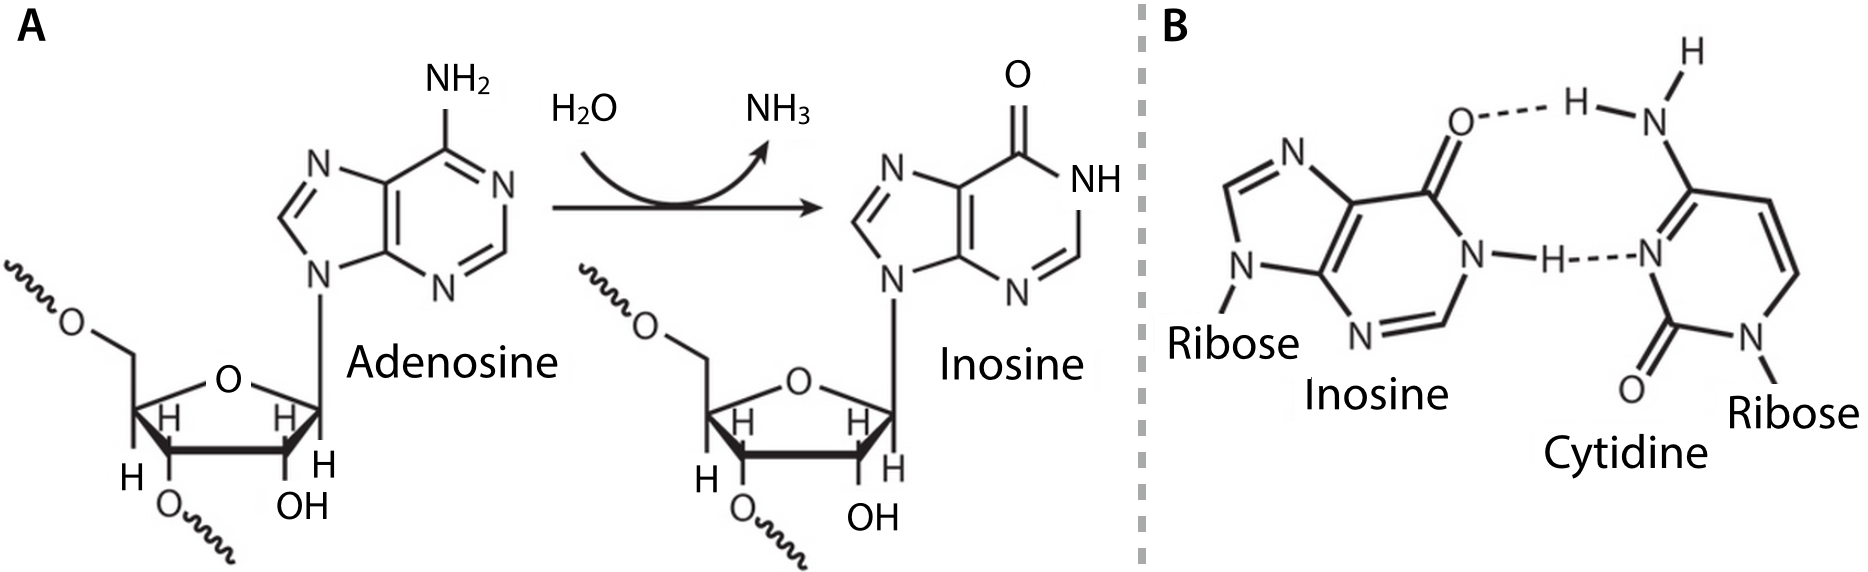
\includegraphics[width=15cm]{Adenosine-inosine.png}
	\end{center}
	\caption{ADARの生化学的な作用機序 (\cite{Nis10}より改変)}
	\begin{flushleft}
		\small{\textbf{A}: ADARによるアデノシンからイノシンへの化学修飾が触媒される様子を示す。アデノシンはADARによる脱アミノ化反応によってイノシンへの一塩基修飾を受ける。イノシンへの修飾は同時に標的となった二本鎖RNAの二次構造を変化させる。\textbf{B}: 編集を受けたイノシンは、シチジンと塩基対を形成する。}
	\end{flushleft}
	\label{fig:Chemical_reaction}
\end{figure}

図\ref{fig:adar_domain}にADARの持つ機能ドメイン構造を示す。ADARはアデノシンからイノシンへの塩基修飾を触媒するdeaminaseドメインと二本鎖RNAに結合するdsRBD (Double-stranded RNA binding domain)の2つの機能ドメインをヒト、マウス、線虫、ショウジョウバエは共通して有する \citep{JinZhaLi0906}。dsRBDは65残基程度の長さの中にα-β-β-β-αという特徴的なドメイン構造を持ち、直接的に二本鎖RNAと接触するためA-to-I編集に必須の機能ドメインの一つである \citep{Barraud:2012aa, ChoYanLee0305, LaiDraNis9507}。ヒトのADAR1においては、Z-DNA-bindingドメインを1つから2つ有しているが、これはADARのターゲットとなる転写物、特にsiRNAなど短鎖の二本鎖RNAとの結合における親和性を高めるためだと考えられている \citep{QiZhaQiu1205}。また、ヒトのADAR3のみに特徴的にアルギニンリッチな一本鎖RNA結合ドメインのR-domainを持つが、この生物学的な意義については明らかにされていない \citep{CheChoWan0005}。ヒトの2つのADAR1、L型とS型はスプライシングアイソフォームとして知られ、それぞれ異なるプロモーターから転写されることが分かっている \citep{KawSam0011}。\textit{in vivo}では、ADAR1およびADAR2はホモダイマーの形成が脱アミノ化反応には必須であることが報告されている \citep{GalKeeRin0307}。
\par
ADAR1およびADAR2は、真核生物における昆虫やイカ、脊椎動物など進化的に広く分布し、高い配列保存性を示す。酵母や原生生物、植物においては発見されていない。ヒトにおいては、これまでにADAR1、ADAR2、ADAR3の3種類が同定されている。このうち、ADAR1およびADAR2は酵素活性が確かめられているが、ADAR3に関しては機能ドメインは保存されているものの、脱アミノ化活性については不明である \citep{Nishikura:2006aa, MelMaaHer9612}。また、ADAR3は、脊椎動物のADAR2の遺伝子重複により生じたとも考えられている \citep{JinZhaLi0906}。

\begin{figure}[!h]
	\begin{center}
		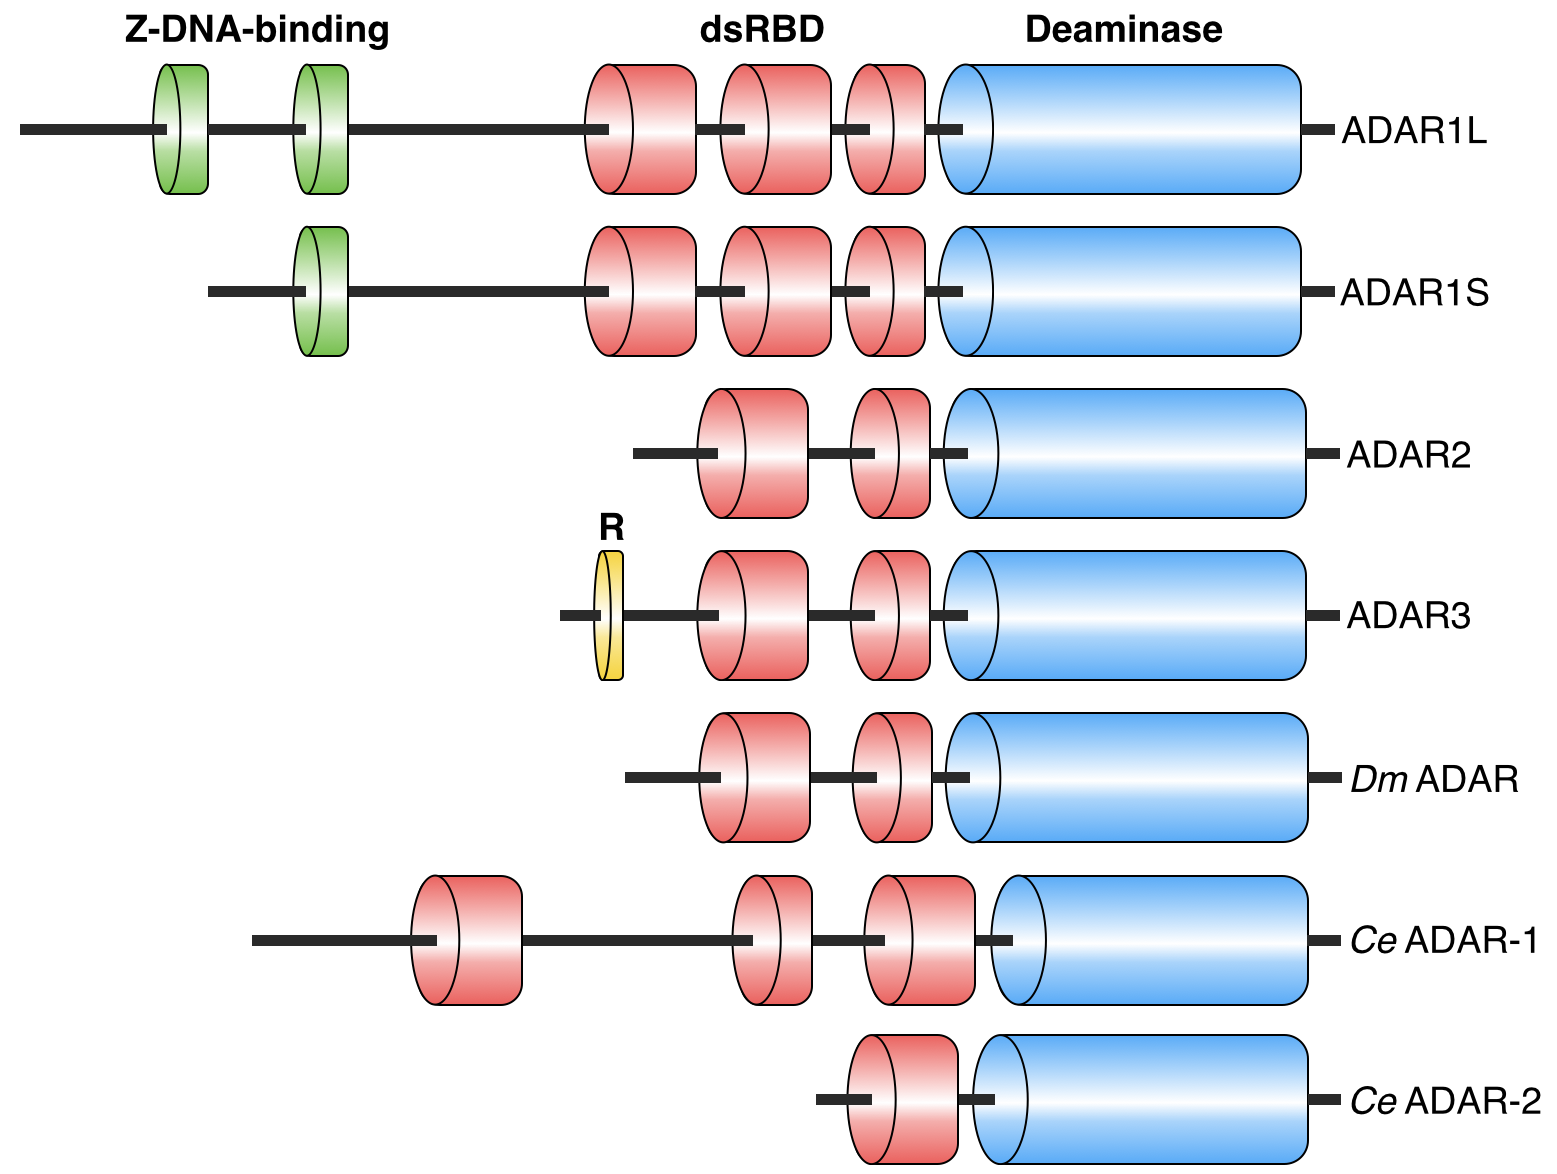
\includegraphics[width=11cm]{Adar_domain.png}
	\end{center}
	\caption{ADARタンパクのドメイン構造}
	\begin{flushleft}
		\small{ヒト、線虫、ショウジョウバエにおけるADARのスプライシングバリアントを含めたドメイン構造を示す。左から順に、Z-binding (緑)、Double stranded RNA binding (赤)、Deaminase (青)、Arginine-rich (黄)の通り、それぞれ機能ドメイン構造ごとに色分けした。上からADAR1L、ADAR1S、ADAR2、ADAR3はヒトから同定されたADARのバリアント、\textit{Dm} ADARはショウジョウバエ、\textit{Ce} ADAR-1、\textit{Ce} ADAR-2は線虫におけるADARである。}
	\end{flushleft}
	\label{fig:adar_domain}
\end{figure}

\subsection{二本鎖RNAの二次構造と修飾塩基の選択性}
ADARによるA-to-I編集は、イノシンへ修飾される位置に高い選択性のある場合と、選択性が低くRNAへランダムに置換する2つのタイプに分類される \citep{Nis10}。位置選択性の高い編集は、20塩基程度の短い二本鎖RNAを形成しADARのターゲットとなるのに対し、ランダムに編集される非選択的な編集サイトは、二本鎖RNAが100塩基以上であることが多く、非選択的な編集は、最大でも50\%程度がイノシンへと修飾される傾向が見られることが報告されている。これまでの研究から、特定のアデノシンが選択的に編集するためには、二本鎖RNAの形成する特異的に二次構造が重要であることが明らかとなっている \citep{LehBas9908}。
\par
古くからA-to-I編集の研究対象となっているグルタミン酸受容体 (Guanosine receptor-2, GluR2)やセロトニン受容体 (Serotonin receptor-2C, 5-HTR)は、編集の入る位置に高い特異性を示し、特定のアデノシンのみが選択的にグアノシンへと置換される。このような位置特異的なA-to-I編集においては、隣接するエクソン-イントロン境界における相補的な配列、ECS (Editing-site complamentary sequence)およびその二次構造の形成が不可欠であることが知られている \citep{HigSinKoh9312}。
\par
GluR2においては、編集サイト毎にADAR1またはADAR2のどちらか一方に優先的に編集されることが知られており、位置毎におけるADARの選択性は、ADARの持つdsRBDの数とドメイン間の配列長の相違がADARと二本鎖RNAとの相互作用を変化させることに起因するとの報告がある \citep{Nishikura:2006aa}。ヒトB細胞において、siRNAによる\textit{Adar1}および\textit{Adar2}のノックダウンを別々に行った解析では、同定されたA-to-I編集のうち、20\%程度が\textit{Adar1}および\textit{Adar2}の共通したターゲットとなっていることが報告されている \citep{Wang:2013aa}。また、\textit{Adar1}のみをサイレンシングした場合、A-to-I編集サイトの総数は1/3程度に減少することから、ヒトB細胞においては\textit{Adar1}によるA-to-I編集が優勢的であると考えられる。図\ref{fig:ADAR}に二本鎖RNAに結合するADARとそのサイトを模式的に示した。

\begin{figure}[!h]
	\begin{center}
		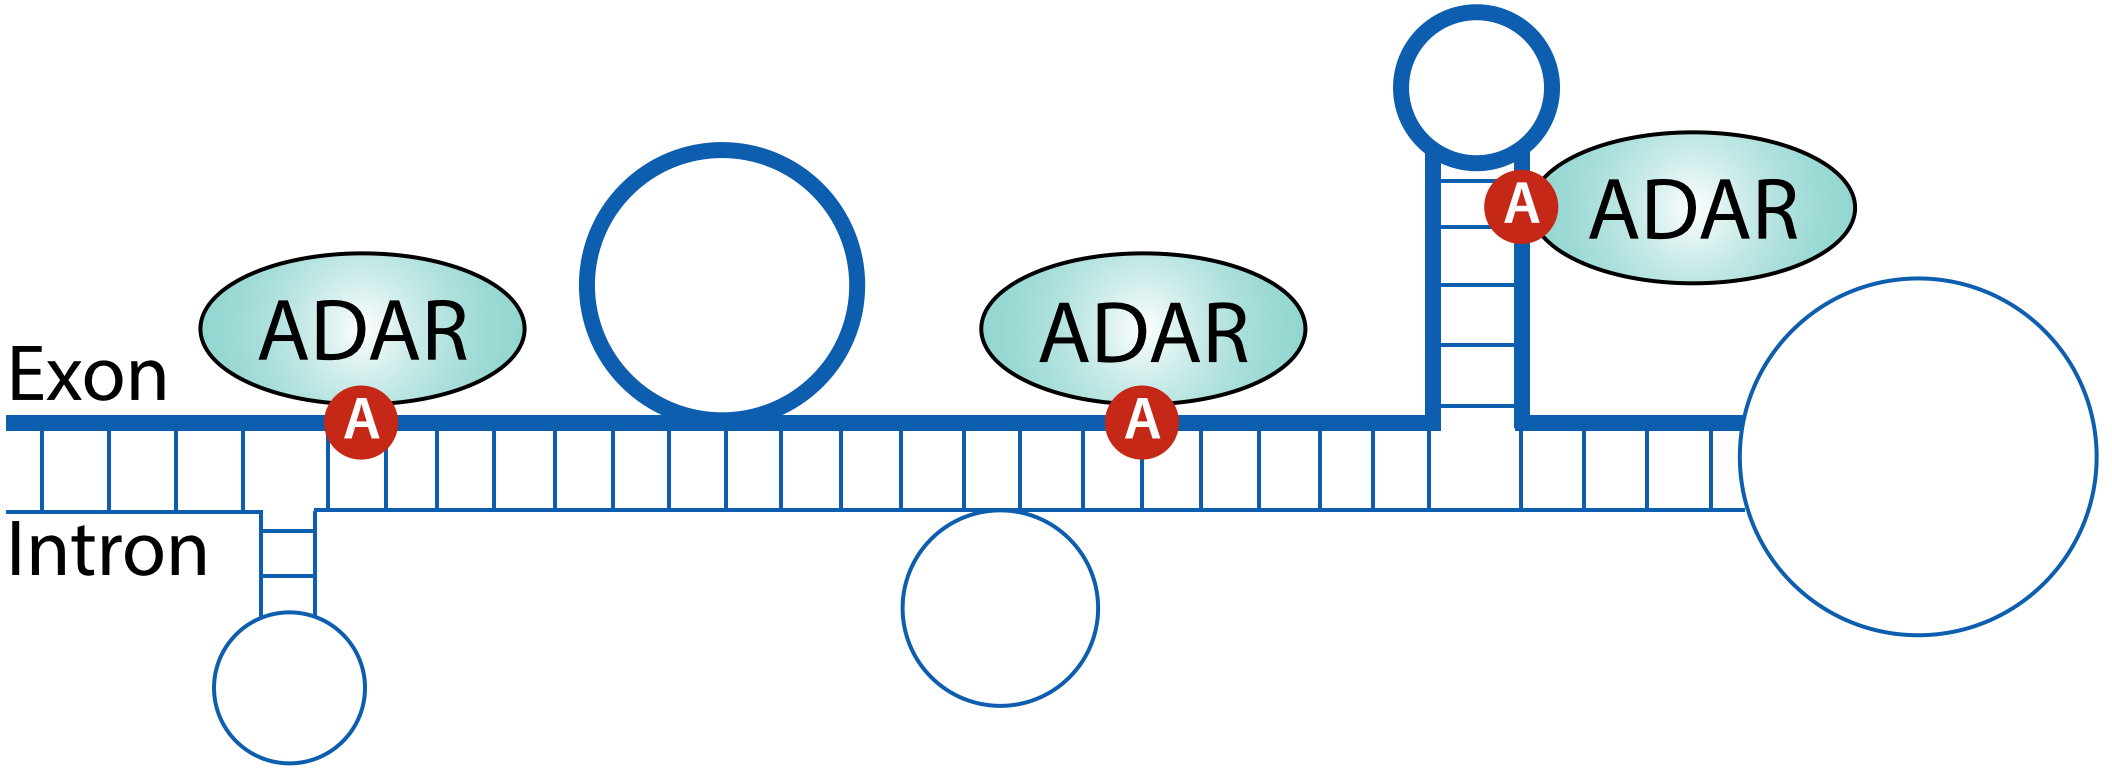
\includegraphics[width=14cm]{ADAR.png}
	\end{center}
	\caption{ADARによるA-to-I編集の模式図}
	\begin{flushleft}
		\small{ADARは二次構造を形成した二本鎖RNAへ特異的に結合し、アデノシンからイノシンへの塩基置換を触媒する。多くの転写物は複数の編集サイトを持つことが知られる。エクソン領域 (太線)に隣接するイントロン領域 (細線)の間に二次構造が形成され、3箇所に編集が起きている様子を表す。}
	\end{flushleft}
	\label{fig:ADAR}
\end{figure}

\subsection{\textit{Adar}遺伝子の欠損による生理学的な影響}
生体内における\textit{Adar}の発現が生理学的に重要な役割を持つことは、ヒトやマウス、線虫などの変異株や遺伝子サイレンシングを用いた実験により明らかにされてきた。ショウジョウバエにおいては、\textit{Adar1}の欠損により、協調的な運動行動の欠損や加齢依存的な神経変性が報告され \citep{PalKeeOCo0008}、線虫においては\textit{Adar1}および\textit{Adar2}のホモ変異体は、走化性が欠損することが報告されている \citep{TonSacMor0211}。マウスにおける\textit{Adar1}および\textit{Adar2}はともに致死性を示す。\textit{Adar1}の変異体では初期発生段階において赤血球新生における異常によるアポトーシスが原因で致死の表現型を示し \citep{HarWalLu0901}、\textit{Adar2}の欠損は、生後20日以内にけいれん重積により死に至る \citep{HigMaaSin0007}。この原因は、グルタミン酸受容体における編集不全を原因とすることが分かっている。ヒトにおいては、ADARによる編集不全に起因した疾患が報告されており、\textit{Adar1}のホモ変異体は、遺伝性対側性色素異常症を引き起こす他、グルタミン酸受容体における不完全な編集は、筋萎縮性側索硬化症の原因となることが明らかとなっている \citep{MiySuzKon0309}。また、未編集のセトロニン受容体が精神疾患の原因となることも指摘されている \citep{Slotkin:2013aa}。

\subsection{ADARの発現と細胞内局在}
ADARは核内と細胞質のどちらにも局在することが知られる。ADAR1については核内と細胞質に局在するADAR1LおよびADAR1Sが知られるほか \citep{PatSam9510}、ADAR2は核に局在することが知られる \citep{DesKeeLaf0305}。また、ADAR3は脳特異的に発現していることが知られる \citep{MelMaaHer9612}。核内で起こるA-to-I編集は、RNAポリメラーゼIIによる転写と同時、すなわちCo-transcriptionalに作用していることがショウジョウバエにおける核内の新生RNAを用いたトランスクリプトーム解析から報告されている \citep{Rodriguez:2012aa}。Co-transcriptinoalなA-to-I編集は、スプライシングの効率に影響を与えているデータも示されており \citep{Laurencikiene:2006aa}、ADAR1およびADAR2の細胞内局在とスプライシング機構との関係性については、今後より詳細が明らかにされるだろう。
\par
ADAR2は自己編集 (self-editing)と呼ばれる機構が知られており、発現しているADAR2のmRNAに対して数カ所のA-to-I編集を起こす \citep{GanZhaYan0611}。結果として、ADAR2-mRNAは4番イントロンと5番エクソンとの間に47塩基が挿入されたフレームシフト変異を引き起こし、新しいスプライスバリアントは編集活性を持たないことが報告されている \citep{HanTohMat0808}。このことは、ADAR2が自身の活性をA-to-I編集により制御するという非常に興味深い現象である。
\par
ヒトの8つのセルラインを用いて、核内と細胞質を分離したRNA-seq解析からは、核内で起こるA-to-I編集が細胞質で起こるものより数倍以上高頻度である傾向が見られることから、A-to-I編集の多くはCo-transcriptionalに起きていることを示唆していると考えられる。核内と細胞質ともに70\%がセルライン特異的なA-to-I編集を占めることが報告されている \citep{Che1307}。

\subsection{RNA編集の進化的な起源と意義}
A-to-I編集による塩基修飾は、現存する生物が祖先種の遺伝子配列を獲得する復帰突然変異としての役割を持つという仮説が提唱されている \citep{Che1307, Pinto:2014aa}。\cite{Che1307}は、ヒト、チンパンジー、アカゲザルのゲノム配列から祖先種のゲノムを推定し、ヒトゲノムと推定した祖先種ゲノムの塩基配列を比較すると、ヒトの90\%以上のA-to-G 編集サイト (=グアニン)は祖先種においてもグアニンであることを示した。このことは、進化の過程でアデニンへの一塩基置換が起こり、再びその箇所をA-to-G 編集を起こすことにより、祖先配列を獲得している可能性が持たれている。このようなA-to-G 編集による復帰突然変異のような現象を\cite{Che1307}はRNA memoryとして提唱している。しかしながら、現存しない祖先種のゲノム配列を検証することは難しく、祖先配列との比較結果は見かけ上の現象なのか、RNA memoryが何らかの制御を受けた結果であるのかは議論の余地があると考えられる。

\section{A-to-I編集の持つ多様な生理学的機能}
\subsection{タンパク機能の調節と多様化}
真核生物におけるRNA編集の重要な役割として古くから認識されてきたものは、翻訳領域内におけるアミノ酸配列の変化を伴ったA-to-I編集である。AMPA型グルタミン酸受容体は、GluR2サブユニットは他のサブユニットに対して膜上のアミノ酸がグルタミン (Q)から陽電荷を有するグリシン (R)へと変化しており、その結果としてGluR2サブユニットを有するAMPA型グルタミン酸受容体のみ、カルシウムに対する非透過性を示す \citep{HigSinKoh9312}。このカルシウム透過性に関する制御はQ/R調節とも呼ばれ、A-to-I編集によるグルタミン (CAG, Q)からグリシン (CIG, R)への非同義置換によって達成されている。哺乳類の神経細胞においては、100\%に近い割合でQ/R調節が行われており、RNA編集率の低下は細胞内へのカルシウムの透過率をさせ、結果として細胞死やヒトの場合は疾患の原因となることが報告されている \citep{Slotkin:2013aa}x。
\par
タコの遅延整流性のカリウムイオンチャネル$K_{V}$は、14箇所の編集が起こることが発見されている \citep{Garrett:2012aa}。この編集を受けたK$_{V}$1.1チャネルへの4箇所のA-to-I編集は、イソロイシンからバリンへの非同義置換を引き起こし、ゲートの開閉を加速させることが報告された。寒冷性のタコは、編集を受けることにより、温帯性のタコよりも低い温度での活動を可能にしていることが示唆されている。

%\subsection{非翻訳RNAへのA-to-I編集}
%これまでは、GluR2やK$_{V}$チャネルなど、翻訳領域の特定のグアノシンを選択的にイノシンへ置換することによるA-to-I編集の生理学的な影響を概観してきた。ところが、ESTs (Expression Sequence Tags)配列や超並列シーケンサーによるA-to-I編集の網羅的な観察が可能になると、LINEやSINE、Alu配列などの反復配列、またUTRやイントロンなど非翻訳領域における編集が全体の80\%以上を占めるという傾向が今日では明らかとなってきた。こういった背景から、遺伝子領域をターゲットとしたA-to-I編集に加えて、反復配列や非翻訳RNAとA-to-I編集の関係性についての解析が一挙に推し進められるようになった。
%\par
%興味深いことに、A-to-I編集は、核内外においてDicerやDrosha、RISCなどRNA結合タンパク複合体や、miRNAやsiRNAなど、他の二本鎖RNAと相互作用を起こすことが明らかとなってきた。こういった現象は、A-to-I編集がタンパク質の機能を多様化させる他に、真核生物においては非翻訳領域におけるA-to-I編集を介した積極的な遺伝子発現制御を行う可能性を示唆する知見である。

\subsection{二本鎖RNAの安定性への寄与}
ADARによるA-to-I編集は、二本鎖RNAが形成する折りたたみ構造を局所的、また大域的に変化させる。RNA分子における塩基対形成は、I:UおよびG:Cのワトソン・クリック型塩基対で安定的に形成するが、A-to-I編集により一般的なワトソン・クリック型塩基対ではなく、I:Uがペアリングするゆらぎ塩基対 (Wobble base pair)を形成する \citep{Barraud:2012aa}。このゆらぎ塩基対は、二本鎖RNAを熱力学的に不安定化させる。この逆に、A:Cなどのゆらき塩基対に対するA-to-I編集は、二本鎖RNAの安定化に寄与すると考えられる。このように、A-to-I編集による塩基対形成の変化は、局所的または大域的に二本鎖RNAの安定性を変化させると考えられている \citep{Nis10}。

\subsection{スプライシング機構との関連性}
真核生物のほぼ全てのエクソン-イントロン境界は、GU-AG配列と呼ばれる強いコンセンサス配列が保存されており、スプライシング機構においてイントロンとエクソンの境界を決めている \citep{Graveley:2001lq}。3'スプライスサイトはドナーサイト (donor site)、5'スプライスサイトはアクセプターサイト (acceptor site)と呼ばれ、AU配列またはAG配列へのA-to-I編集はそれぞれ新生のアクセプターサイト、ドナーサイトを形成する。また、AG配列へのA-to-I編集は、3'スプライスサイトを欠失することがこれまでに報告されている \citep{ValNis05}。また、このようなスプライスサイトの新生や欠失が二本鎖を形成したAlu配列に起こる場合、Alu配列の一部がエクソン化 (exonization)し、mRNAに新たなエクソンとして取り込まれる例がヒトのNuclear prelamin A recognition factor (NARF)タンパクでは知られている (図\ref{fig:Alu_adar}) \citep{SorLevRez0404}。A-to-I編集によるAlu配列のエクソン化は、新たな機能を持つタンパク質のバリアントを生み出すため、進化的に重要な役割を担っていると考えられている。

\begin{figure}[!h]
	\begin{center}
		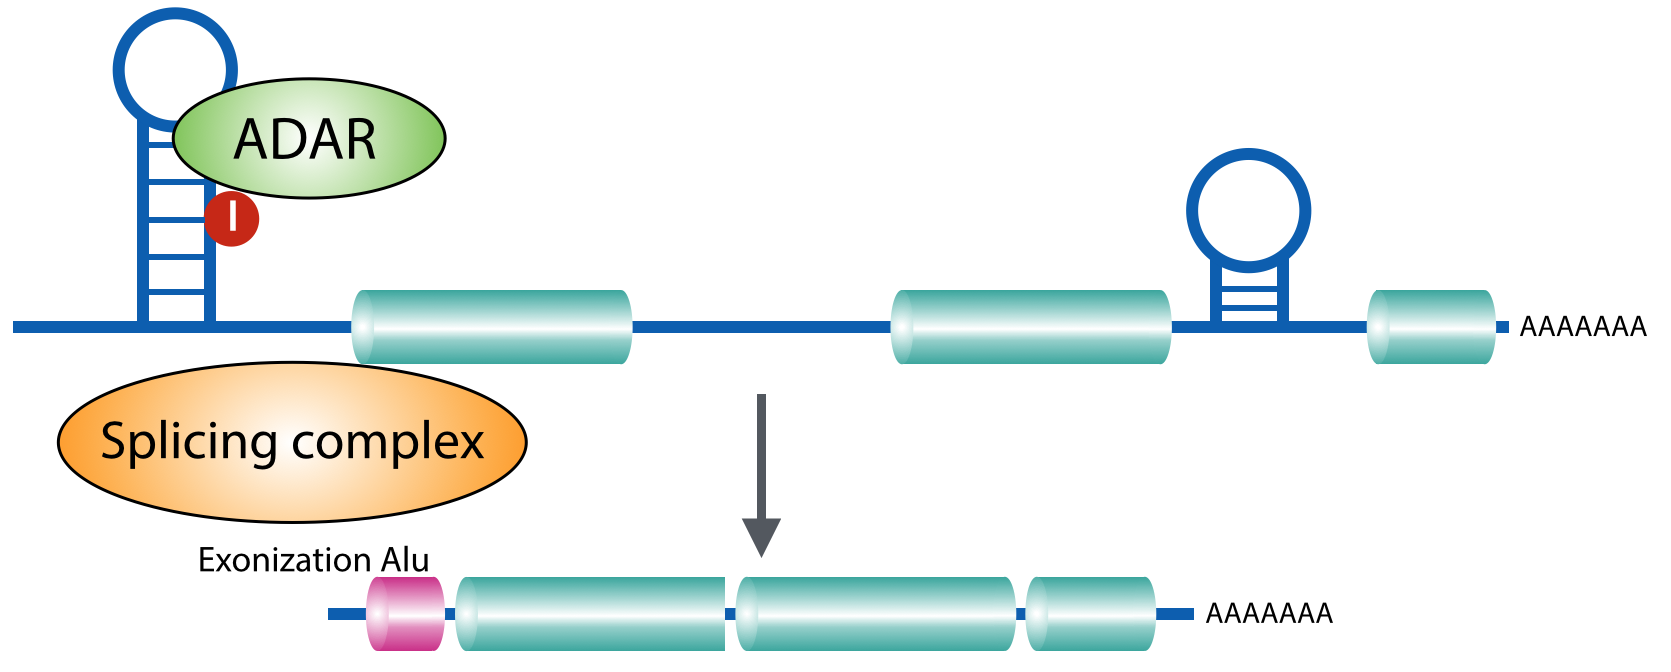
\includegraphics[width=14cm]{Alu_adar.png}
	\end{center}
	\caption{A-to-I編集によるAlu領域のエクソン化 (\cite{Nishikura:2006aa}より改変)}
	\begin{flushleft}
		\small{イノシンは、スプライシング機構においてグアノシンとして認識される。二本鎖RNAを形成したAlu配列を標的としたA-to-I編集は、GU配列やAG配列といったスプライスサイトを新生あるいは欠損させる。スプライスサイトの新生と欠損は、Alu配列の構成性エクソン (Constitutive exon)へのそれぞれ取り込みと排除を起こす。}
	\end{flushleft}
	\label{fig:Alu_adar}
\end{figure}

\subsection{miRNAへの編集と遺伝子発現制御}
低分子RNA (Small RNA)の一種として知られるmiRNAは、複数のRNA結合タンパクと相互作用し、転写されたmRNAに対して分解を促進し、遺伝子の翻訳抑制を行う真核生物において重要な低分子RNAの一つである \citep{KroLoeFil1009}。miRNAは、初めは数百から数千塩基程度のpri-miRNA (primary-miRNA)として転写されDrosha-DGCR8複合体によりヘアピン構造のpre-miRNAとして切り出され、細胞質へ輸送される。細胞質では、pre-miRNAはDicer-TRBP複合体による切断を受けた後に、21塩基程度の二本鎖RNAとなり成熟する。miRNAは、RISC (RNA-induced silencing complex)へと取り込まれ、標的となった遺伝子の3'末端の非翻訳領域に結合し、mRNAの分解に作用する \citep{CarSon0902}。

\begin{figure}[!h]
	\begin{center}
		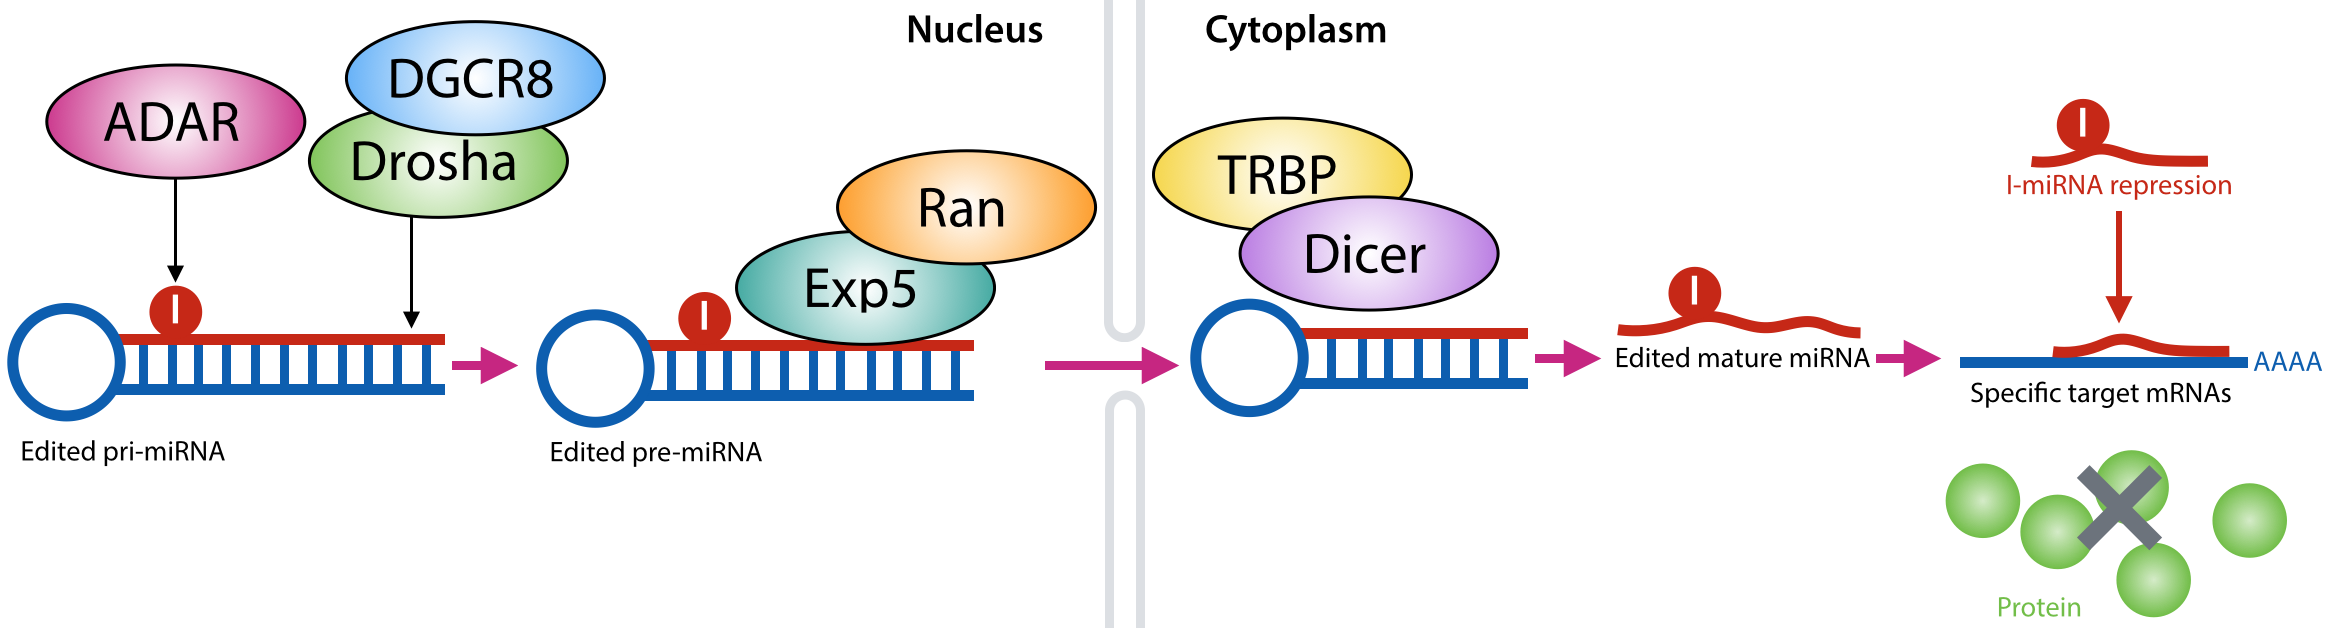
\includegraphics[width=16cm]{miRNA.png}
	\end{center}
	\caption{miRNAへのA-to-I編集による遺伝子発現調節}
	\begin{flushleft}
		\small{miRNAが核から細胞質へ輸送され、成熟して機能する経路を示す。miRNAは、成熟過程においてA-to-I編集を受ける。Drosha-DGCR2複合体やTRBP-Dicer複合体における切断部位の近傍へのA-to-I編集は、miRNA産生量の増加と減少に影響している。シード配列への編集は、標的となる遺伝子を変化させることが知られる。}
	\end{flushleft}
	\label{fig:miRNA}
\end{figure}
pri-miRNAからmiRNAへと成熟する過程では、二本鎖RNAを形成するためDroshaやDicerによる切断と同様にADARによるA-to-I編集もその標的となる。ADARが二量体で機能する場合、ADARによるpri-miRNAへの編集は大きく3タイプに分類することができる。一つ目は、pri-miRNAのDroshaによる切断部位の近傍に編集が入ることで、pri-miRNAは切断されずにイノシン特異的に認識するTudor-SN (Tudor Staphylococcal
Nuclease)による分解を受ける。二つ目は、pri-miRNAがDicerの切断部位の近傍に編集が入ることで、Exportin-5 (Exp5)を介して細胞質へ輸送されるが、Dicerへの切断に抵抗性を示すため、成熟せずmiRNAは機能しない。三つ目は、正常なmiRNAとして成熟するが、厳密にターゲットを識別するシード配列に編集が入ることにより、標的遺伝子が変化する場合である \citep{Slotkin:2013aa}。
\par
最近では、ADARとDicerが複合体を形成し、miRNA産生の活性化にもADARが関与していることが明らかとなってきた \citep{OtaSakGup1304}。ADAR-Dicer複合体は、A-to-I編集能を持たないことも明らかとなっており、miRNAの合成経路とADARの多様な関係性が明らかにされている。

\subsection{siRNA産生の制御とRNAi経路とのクロストーク}
miRNAの生合成過程におけるA-to-I編集と同様に、Dicerのよる切断を受けて成熟するsiRNA (small interfering RNA)もまたA-to-I編集の影響を受けていることが明らかとなっている \citep{YanWanHow0502}。siRNAはDicerによって21塩基から24塩基程度の二本鎖RNAへと切断され、miRNAと同様にRISCを形成する。RNAi経路においては、siRNAと相補的な配列を有する遺伝子が転写抑制の標的となるため、Argonauteタンパクなどの複合体としてRISCに取り込まれたsiRNAは標的遺伝子を認識する重要な役割を持つ \citep{Fil0507}。

\begin{figure}[!h]
	\begin{center}
		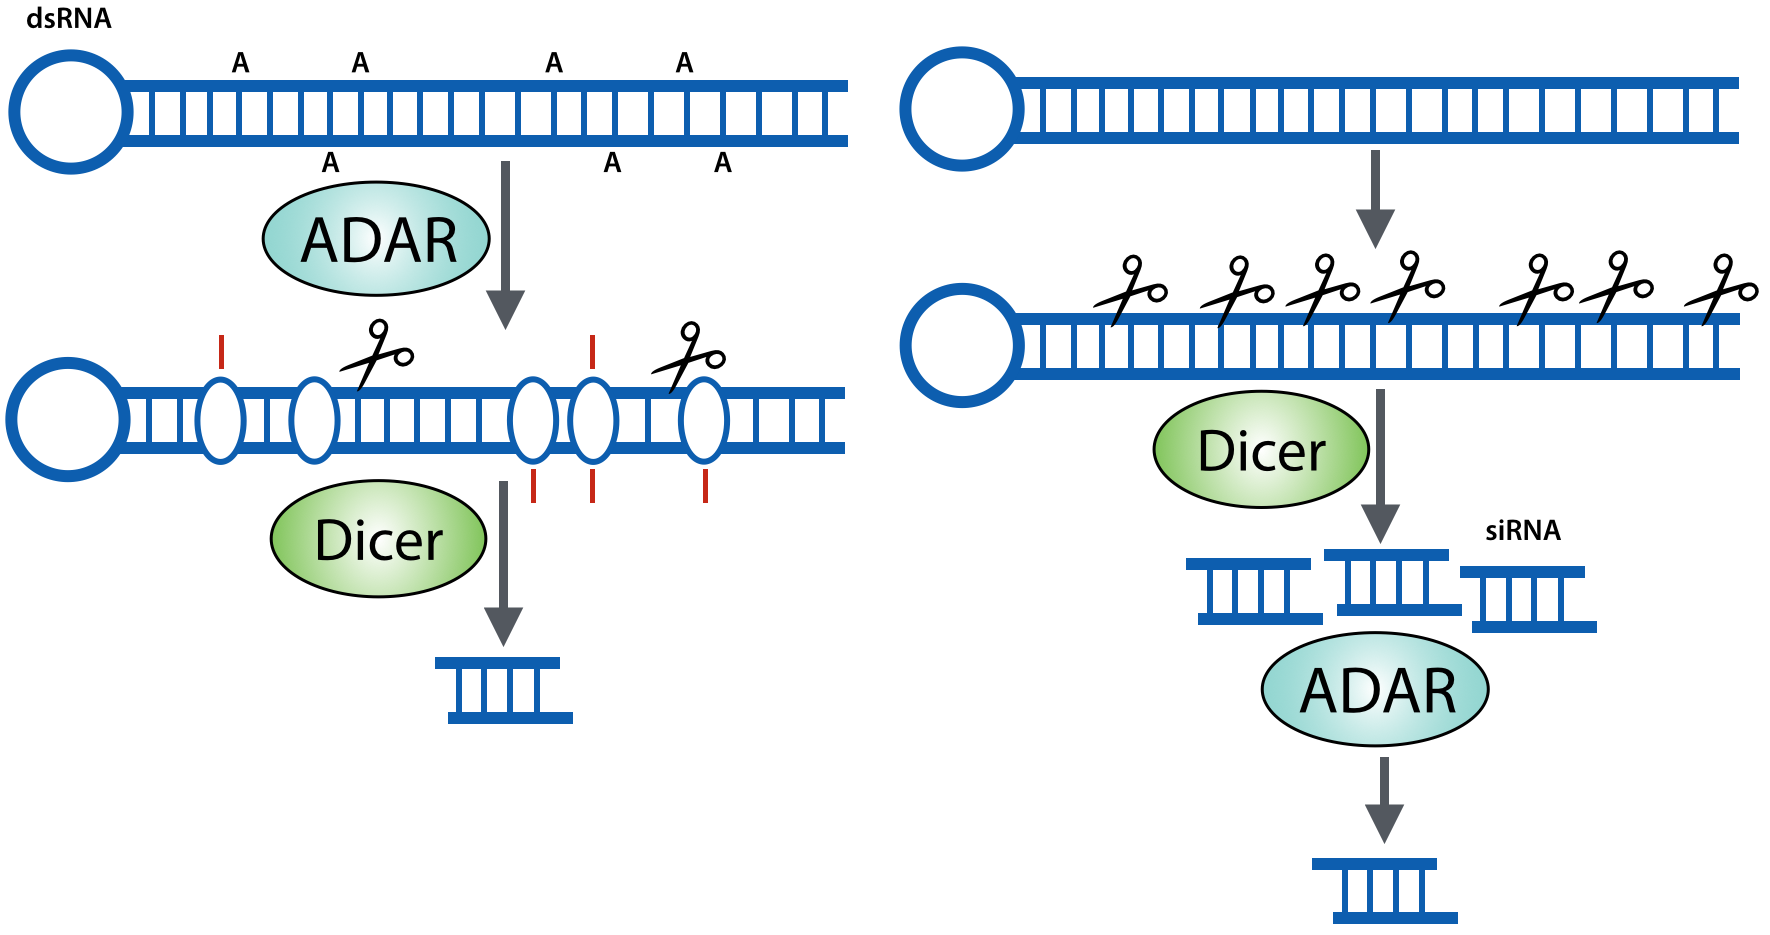
\includegraphics[width=14cm]{siRNA.png}
	\end{center}
	\caption{ADARによるsiRNAの制御とRNAi経路への影響}
	\begin{flushleft}
		\small{長鎖非翻訳RNAは、Dicerによる切断を受けて内在性siRNAとして機能する。現在考えられているA-to-I編集によるsiRNAの制御を左右にそれぞれ示した。左は、A-to-I編集を受けた長鎖ヘアピン二本鎖RNAへのがDicerへの切断抵抗性を示すために、内在性siRNAの産生量が減少する場合である。右は、既に生成されたsiRNAに対して、細胞質に局在するADAR1が強く結合することにより、siRNAのRISCへのローディングを阻害し、siRNA濃度を減少させる場合である。}
	\end{flushleft}
	\label{fig:adar_siRNA}
\end{figure}

このように、RNAi経路においてDicerとADARは共通して二本鎖RNAを標的とするため、siRNAのDicerの切断部位へのA-to-I編集はRNAi経路へ拮抗的に作用する。線虫においては、ADARによるsiRNAへの編集がRNAi経路を阻害し、遺伝子発現へ影響を及ぼすことが報告されている \citep{KniBas0210}。
\par
ウィルスなど外来性RNAに由来するsiRNAに加えて、マウスの卵母細胞を用いた実験では、SINEなどレトロトランスポゾンが形成する長鎖ヘアピン (lhRNA, long-hairpin dsRNA)二本鎖RNAがDicerの標的となって、内在性siRNA (endogenous siRNA)が生成する経路が報告された \citep{Watanabe:2008aa}。この内在性siRNAは、トランスポゾン活性に対して抑制性に機能するsiRNAである。\textit{in vitro}の実験結果から、A-to-I編集を受けた内在性siRNAはDicerによる切断に対して抵抗性を示すことが分かった \citep{ScaSmi0112}。A-to-I編集によって二本鎖RNAは、A:IからA:Uへ塩基対形成が変化する。A:U塩基対は、Dicerの切断に対して抵抗性を示すため、A-to-I編集は内在性siRNAの産生量を減少させる、或いは正常に機能しない内在性siRNAの産生の制御にA-to-I編集が関与する可能性を示唆している。加えて、この拮抗的な作用とは真逆に、RNAi経路へ促進する機能も同時にADAR1は有していることが報告された。これは、ADARとDicerがホモ二量体の複合体を形成した場合である。

\section{超並列シーケンサーによるRNA編集サイトの検出とその手法開発}
\subsection{網羅的なRNA/DNA differenceサイトの検出}
ここ数年、超並列シーケンサーに代表される配列決定技術の躍進的な発展は、多サンプルのゲノム (DNA-seq)およびトランスクリプトーム (RNA-seq)のシーケンスを可能にしてきた。RNA編集研究においては、超並列シーケンサーから得られる網羅的で定量性のあるRNA-seqデータやDNA-seqデータを用いることにより、A-to-I編集サイトを検出する情報学的手法が精力的に開発されてきた \citep{pmid21596952, Ramaswami:2012aa, Zhu:2013aa, St-Laurent:2013aa, DilHauGib1304, RamZhaPis1302, Bazak:2013aa, Sakurai:2014aa, Pinto:2014aa, Rodriguez:2012aa, Park:2012aa, Peng:2012aa, Kleinman:2012aa, LagHorMar1304, Che1307, BahLeeLi1201}。超並列シーケンサーから測定されるトランスクリプトームやゲノムの配列情報は、数GBから数百GBの配列データを扱うことになるため、こういった大規模な編集サイトの検出は本質的に情報学的な解析が必須となっている。図\ref{fig:pipelines}に解析の基本的なパイプラインを示した。

\begin{figure}[!h]
	\begin{center}
		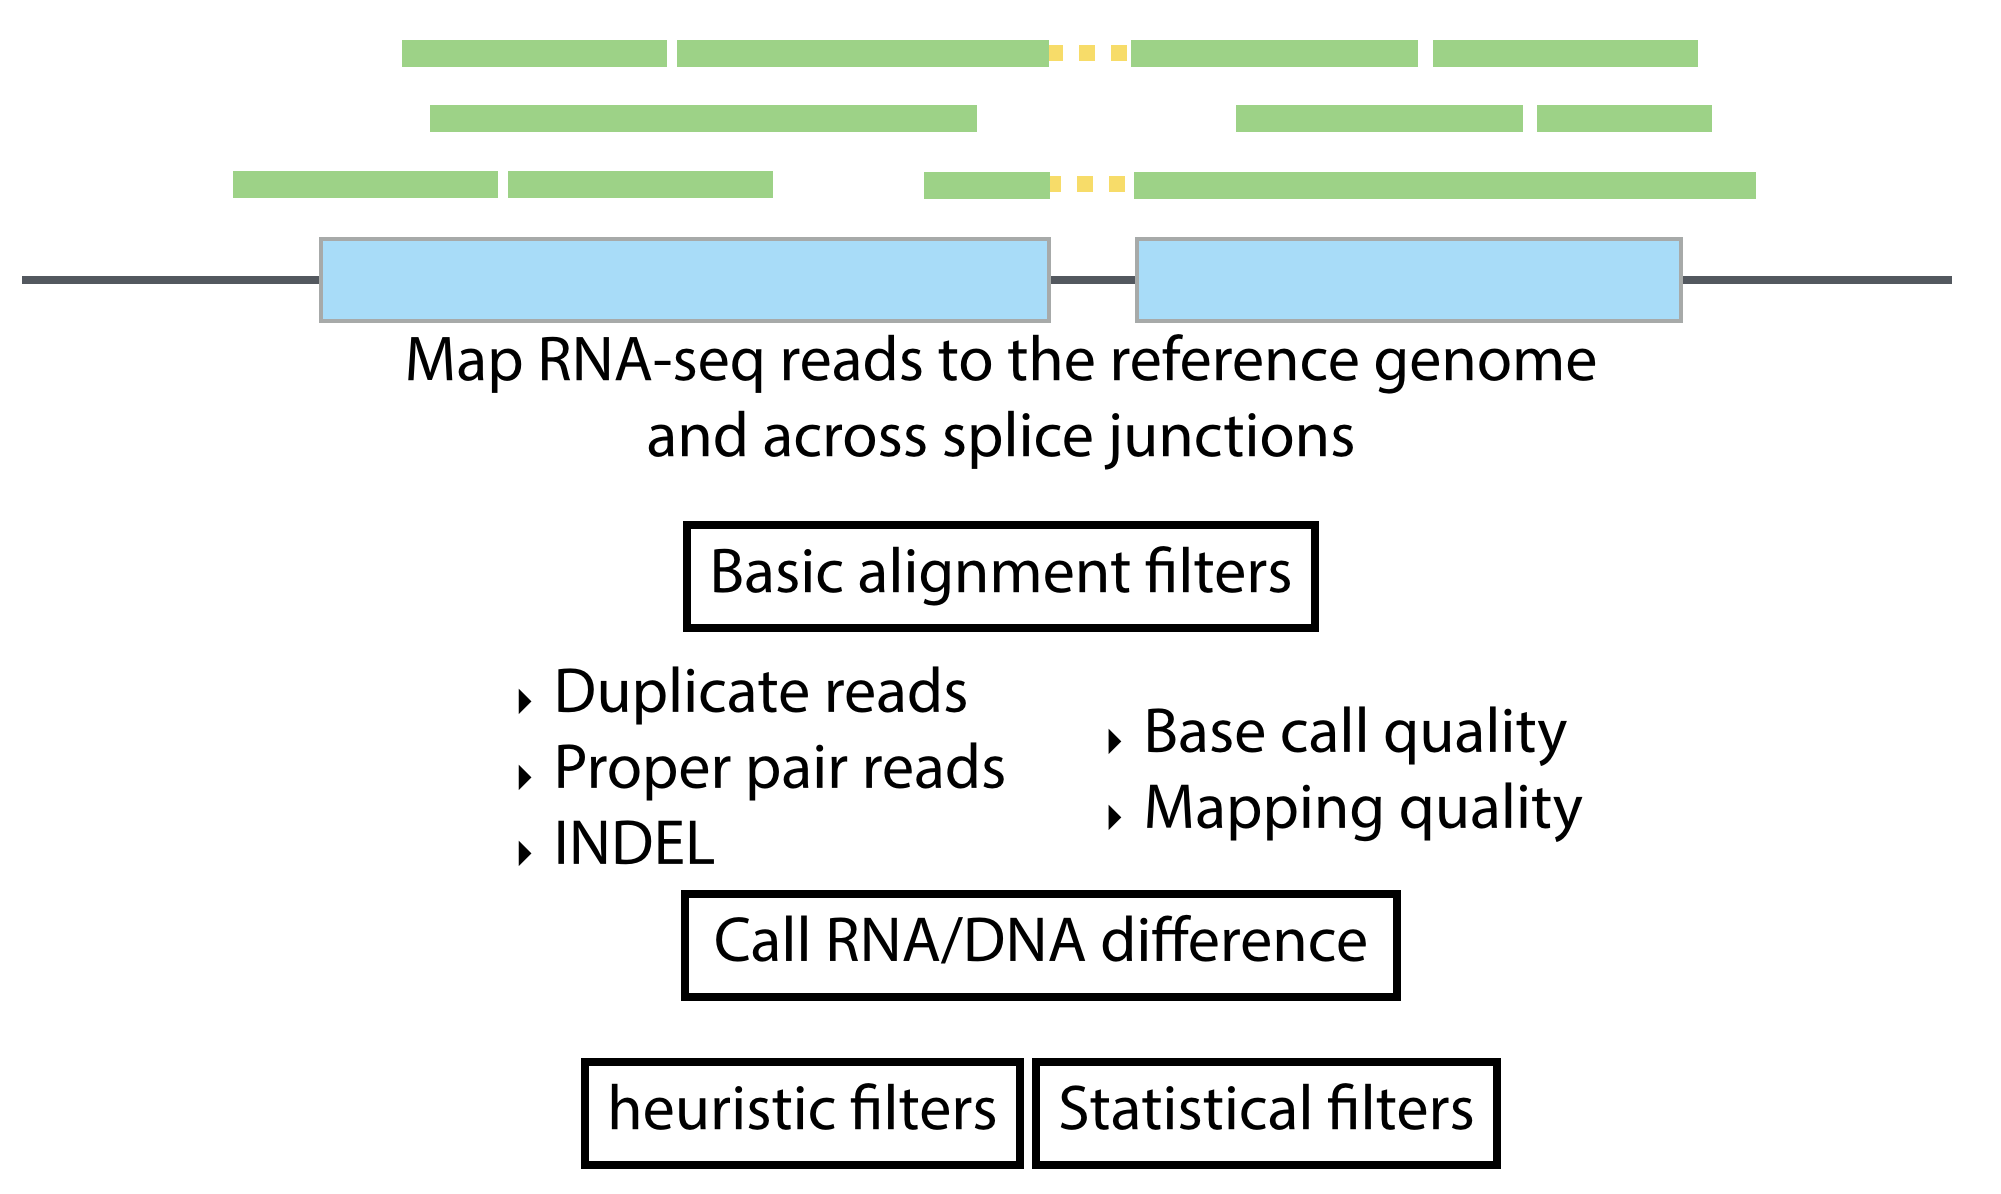
\includegraphics[width=12cm]{pipelines.png}
	\end{center}
	\caption{超並列シーケンサーを用いた基本的なRNA編集サイトの同定手法の解析パイプライン}
	\begin{flushleft}
		\small{超並列シーケンサーから得られたRNA-seqやDNA-seqデータは、まずリファレンスとなるゲノム配列・遺伝子配列へマッピングを行う。次に、カバレッジやマッピングクオリティ、重複リード (PCR duplicated reads)の除外などを行う (pre-filtering処理)。RNA編集サイトは、ゲノム配列との一塩基ミスマッチとして検出することができるため、RNAとゲノム配列の比較を行い、編集サイトを検出する。その後に、SNPやリピート配列、スプライスサイト周辺の編集サイトを排除し、最終的なRNA編集サイトの候補を得る (post-filtering処理)。}
	\end{flushleft}
	\label{fig:pipelines}
\end{figure}

2011年に\cite{pmid21596952}の研究チームは、27個体のヒトのRNA-seqおよびDNA-seqデータから、大量のRDDサイト (RNA/DNA difference site)が検出されたという非常に興味深い研究成果を発表した \citep{pmid21596952}。RDDサイトは、$4\times3$のA-to-G編集を含めた全ての塩基置換のパタンを指す。解析には、B細胞 (immortalized B cell)が用いられ、Illlumina Genome Analyzer IIxによる50塩基の1.1億リードをヒトゲノムにマッピングし、合計で28,000箇所以上のRDDサイトを検出した。10,000箇所以上がエクソン領域におけるRDDサイトであった。ADARによると考えられるA-to-I編集は6,700箇所、APOBECによるC-to-U編集は1,200箇所程度を報告した。また、その他のA-to-C編集やT-to-G編集など修飾酵素が発見されていないRDDに関しては、未知のメカニズムが関与する可能性を示唆した。この結果は、同一個体から得られたゲノムとトランスクリプトームが高頻度で編集を受けている可能性を投げかけた意味において強いインパクトを示した。
\par
ところがこの論文が掲載された後、解析結果に対する4本の追従論文が発表され、\cite{pmid21596952}によって検出された編集サイトの95\%以上は擬陽性の可能性が高いことが指摘された \citep{pmid22422962, pmid22422964, pmid22422963, pmid22022455}。論文では、主にRNA-seqリードを参照ゲノムへマッピングする際のバイアスについて検証が行われ、多くのエラーとその原因が報告された。こういった背景から、\cite{pmid21596952}の研究とその追証は、アラインメントデータへの適切なフィルタリングが編集サイトの正確な検出には極めて重要な過程であることを示し、複数のフィルタリング手法を組み合せたヒューリスティックなRNA編集サイトの検出手法が開発される契機となった。現在では、検出される全体のRDDのうち、A-to-G 編集が80\%以上のデータを示すこと、報告された既知のRNA編集サイトとの一致を示すことが検出手法の妥当性を示す主要な論調となっている。

\subsection{RDDサイトに見られる多種のエラーとバイアス}
\cite{pmid22422963}は、\cite{pmid21596952}のシーケンシングデータを再解析した結果から88\%から93\%が参照ゲノムへのマッピングエラー、シーケンシングエラー、遺伝的な多型に起因した技術的エラー (technical artifacts)だと結論づけた。主要なエラーの原因は、ショートリードのマッピングにおけるpositional biasとstrand biasの二つである。
\par
Positional biasは、RDDサイトをカバーしたショートリードにおける位置の偏りである。$ReadLen$ bpのショートリードにおけるRDDサイトの位置$i$は、$\{i,\ ReadLen-i\}$である。$i$の分布はDNAとRNAの二つのデータに対して同一である、という帰無仮説をt検定により統計的な検定を実施した。結果、8,000箇所のRDDサイトは、ショートリードの両端5bpに極端に集中するというpositional biasが顕著に見られることを報告した。
\par
Strand biasは、RDDサイトをカバーするショートリードの方向 (forward/reverse strand)に見られる偏りである。RDDサイトをカバーするRNAとDNAの2つのデータにリードの向きを加えた(DNA+/DNA-/RNA+/RNA-)4つのクラスに分割し、それぞれ4つのクラスでリード数をカウントする。RDDをカバーするリードとそれ以外のリードにおける方向は、同一であるという帰無仮説に対して、フィッシャーの正確確率検定により偏りを検定した。結果、positional biasと同様に、RDDサイトにおいてはサポートするショートリードの向きがforwardあるいはreverseに有意に偏ること結果が示された。

\begin{figure}[!h]
	\begin{center}
		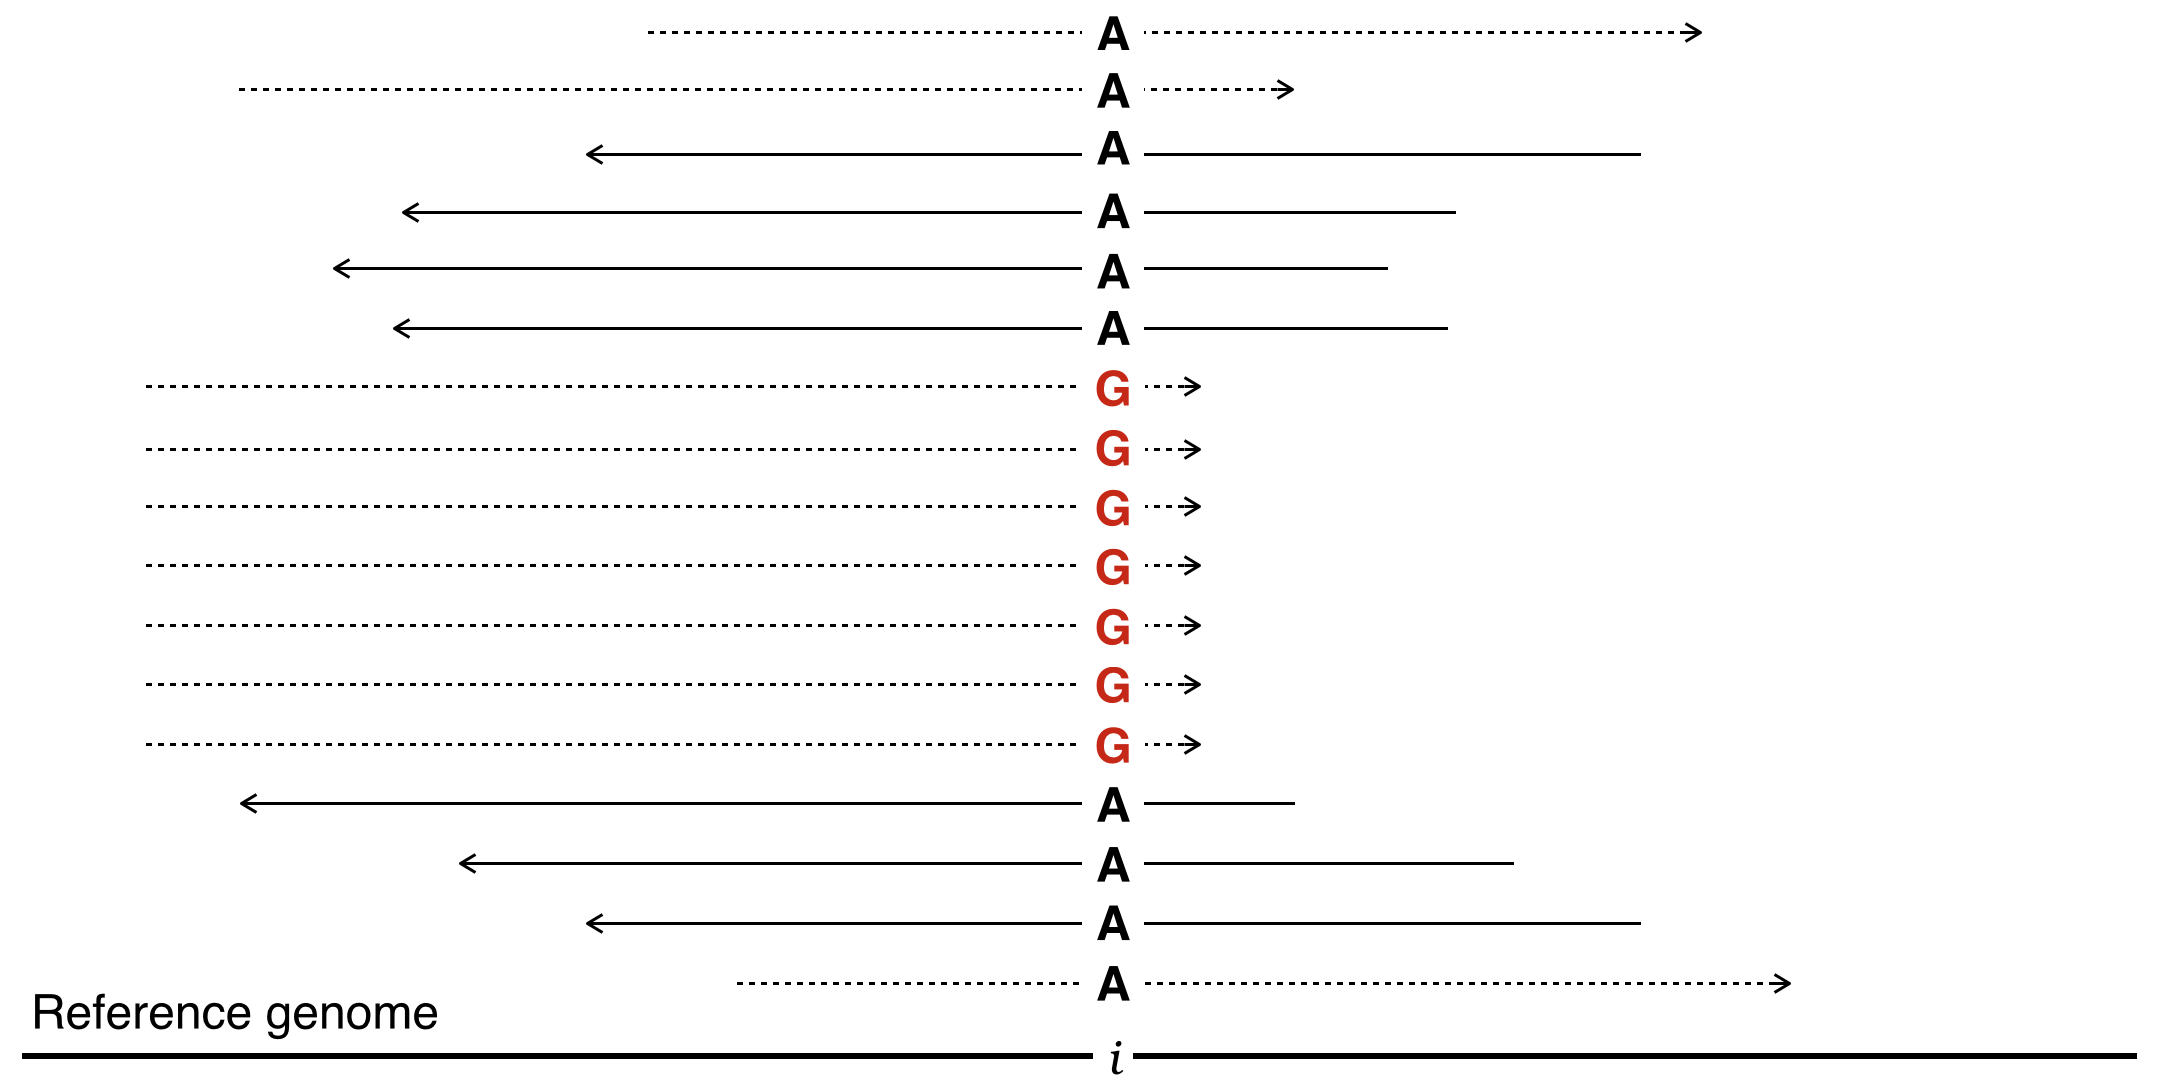
\includegraphics[width=13cm]{pos_bias.png}
	\end{center}
	\caption{検出されたA-to-G 編集サイトに見られるpositional biasおよびstrand bias}
	\begin{flushleft}
		\small{実線はforward strand、破線はreverse strandのショートリードがそれぞれ参照ゲノム配列へマッピングされた結果を表す。黒文字で示したAに対して、ミスマッチ塩基は赤文字のGであることから、A-to-G編集が検出されている。参照ゲノムとマッチしているA塩基は、forwardリードとreverseリードともにカバーされているが、ミスマッチのG塩基はreverse strandのリード (破線)のみからカバーされており、strand biasが見られる。同時にG塩基へのミスマッチは全てのリードが末端の同位置にあり、positional biasが見受けられる。}
	\end{flushleft}
	\label{fig:positional_bias}
\end{figure}

超並列シーケンサーから得られるショートリードの配列は、ゲノム中の反復配列へ適切にマッピングすることが難しく、本来とは異なったゲノム座標へのミスアラインメントの頻度が高くなる \citep{pmid22022455}。誤った座標へのアラインメントを避けるため、BLAST (Basic local search tool) \citep{altschul1990basic}などのローカルアラインメントを行うツールを使い、候補サイトをカバーするショートリードを参照ゲノム配列へ再度アラインメントする (re-alignment)手法がとられている。リアラインメント結果から、ゲノムの複数箇所にマップされたリードを除くことで、候補サイトにに関する精度の高いマッピング結果が得られることが示されている。この反復配列へのマッピングに類似した問題として、splicedアラインメントを行った場合に、エクソンとエクソンの境界のスプライスサイト周辺にミスマッチが集中することが知られている。そのため、既存の遺伝子構造アノテーションを利用し、スプライスサイト周辺の5塩基程度は解析から除外するフィルタリングが行われる場合が多い。加えて、検出された編集サイトが、ADARによる転写後修飾ではなく、SNVやSNPなどゲノム上の変異を反映している可能性が考えられる。そのため、ヒトでは、1000 Genomes Projectなど国際的なプロジェクトによって同定されたSNPのサイトを除外するフィルタリングが行われる。

\subsection{検出された編集サイトの実験的な検証方法}
RNA-seqデータを用いたRNA編集サイトの網羅的な解析は、数千から数万のオーダーで候補を検出する。これらのサイトが真の編集サイトであるかを結論付けるため、現在ではサンガー法による実験的な検証が用いられる場合が多いが、全てのサイトをシーケンシングし直すことはスループットの問題から現実的ではないため、10箇所から100箇所をランダムに抽出し、実験的に検証する場合が殆どである。サンガーシーケンシングにおいても、対象となる編集サイトがゲノムの反復領域に由来する場合、PCRプライマーの特異性が保証されず、編集サイト周辺のみを増幅できない問題がある。これは、\cite{Peng:2012aa}の研究においてサンガーシーケンシングによって検証されたサイトを追証した\cite{Piskol:2013aa}によって指摘されている。追証実験から、反復配列に由来した編集サイトは、PCRバイアスによって正確な検証が行えないことを指摘している。
\par
アミノ酸置換を引き起こす編集の場合には、質量分析器によって得られるペプチド配列のフラグメントから、アミノ酸置換の有無を確認する手法が用いられる \citep{pmid21596952}。この方法は、非同義置換を伴ったコード領域における編集サイトの検証に限られる。

\subsection{A-to-I編集サイトの検出に適切な実験デザイン}
超並列シーケンサーから出力されるRNA-seqデータは、転写物の発現量やスプライシングを考慮した遺伝子構造を推定する用途においては、精度および再現性ともに高く、有用な手法として広く用いられている \citep{MarMasMan0809, MorWilMcC0807}。ところがRNA編集の検出においては一塩基の解像度が求められるため、実験およびデータ解析で混入するノイズの影響を相対的に受けやすくなる。これまでに読み取りエラー (Base call error)の原因として、DNAと比較してRNAは分子として安定性を欠くこと、cDNA合成における逆転写酵素の活性、PCRの配列ごとに見られる増幅バイアス、特定の塩基配列に高頻度の読み取りエラーが発生することなどが指摘されている \citep{NakOshMor1107, AirRosChe11, pmid22099972}。このように、ノイズとADARに由来したA-to-I編集サイトを正確に分離することが、高精度な検出に必要であり、適切に実験をデザインし、シーケンシングデータを取得する必要がある。既往の研究においても、精度の高い検出手法の開発を成功させているものは、情報学的解析のみならず、実験デザインにも優位性が見られる。
\par
先行研究では、カバレッジが10$\times$以上、75塩基以上のリード長、paired-endシーケンシングが事実上の標準となっている。加えて\cite{Ramaswami:2012aa}や\cite{Peng:2012aa}、\cite{Zhu:2013aa}らの解析では、転写物の向きを考慮したstrand-specific RNA-seqが用いられており、センス鎖とアンチセンス鎖を分離した解析を行っている。転写物の方向性を考慮することは、塩基置換のパタンをより正確な分類を可能にする。\cite{Rodriguez:2012aa}らによる解析では、生物学的レプリケートを2サンプル用意し、G検定による統計的な検出手法が用いられている。また、\cite{BahLeeLi1201}や\cite{Rodriguez:2012aa}らのハエやショウジョウバエにおける解析では、\textit{Adar}変異体を同時にシーケンシングし、ADARの発現時のみ見られたA-to-I編集サイトの検出を行っている。ただし、マウスなど\textit{Adar}の変異体が致死性を示す場合には適用が不可能である。また、対象生物種やセルラインのトランスクリプトームと同時にゲノム配列のシーケンスにより、編集サイトがゲノム上のSNV (Single nucleotide variant)などの変異を反映しているか否かを判断可能となるため、多くの研究で用いられている。
\par
ここ数年、ADARによるA-to-I RNA編集に関する研究は、目まぐるしい進展を遂げている。真核生物において発見当初こそ、ランダムで生物学的意義については不明であった非翻訳領域におけるRNA編集であったが、今日では遺伝子の多様な発現制御、スプライシング機構へも影響しているというRNA編集の役割を大きく拡張し、新しい描象が解き明かされつつある。このような現象を貫いているのは、ADARおよびADARと相互作用するDicerやDroshaといった他の因子もまた二本鎖RNA結合タンパクということである。今後、ADARと二本鎖RNA結合タンパクの相互作用は、実験と情報解析の両側から更に研究されることで、ADARの新たな機能は次々と発見されることが予想される。二本鎖RNA結合タンパクとの相互作用を介したADARの理解は、真核生物におけるRNA編集の意義を解き明かす今後の大きな流れとなるであろう。
\par
こういった背景から、大規模な超並列シーケンスデータからノイズと生物学的背景に由来する事象とを精度よく分離可能な実験デザインと情報学的手法を組み合わせた解析の重要性は、今後さらに高まることが予想される。
